\begin{frame}
\frametitle{Implementation}
We choose several representative LSH schemes, implement them and compare their performance.
\begin{multicols}{2}
\begin{itemize}
	\item Basic LSH
	\item LSH Forest
	\item Multi-ProbeLSH
	\item Bayesian LSH
\end{itemize}
\end{multicols}

\textbf{Dataset}. We use MNIST\footnote{http://yann.lecun.com/exdb/mnist/} to evaluate the algorithms. We choose 50 dimensions of the original $28\times28$ images with largest variances as ~\cite{gan2012locality} does. Ground truth are got by linear scan in the training set with Euclidean distance.
\end{frame}

\begin{frame}[shrink]
	\frametitle{Experiment Settings}
	\begin{table}
		\begin{tabular}{ccccc}
			\hline
			Algorithm & Basic & LSHForest & MultiProbe & Bayesian \\ \hline
			\#compounds & 8 & 25 & 8 & \\\hline
		\end{tabular}
	\end{table}
\end{frame}

\begin{frame}[allowframebreaks]
\frametitle{Error Ratio}
Error ratio indicates the accuracy of LSH's results and the ground truth.
Error ratio is close to 1 means this LSH scheme successfully find the nearest neighbors.
	\begin{equation}
		\text{Error Ratio}=\frac{1}{N}\frac{1}{K}\sum_{n=1}^{N}\sum_{i=1}^{K}\frac{d(q, p_{lsh}^{(i)})}{d(q, p_{label}^{(i)})}
	\end{equation}
	
We use $K=20$.

	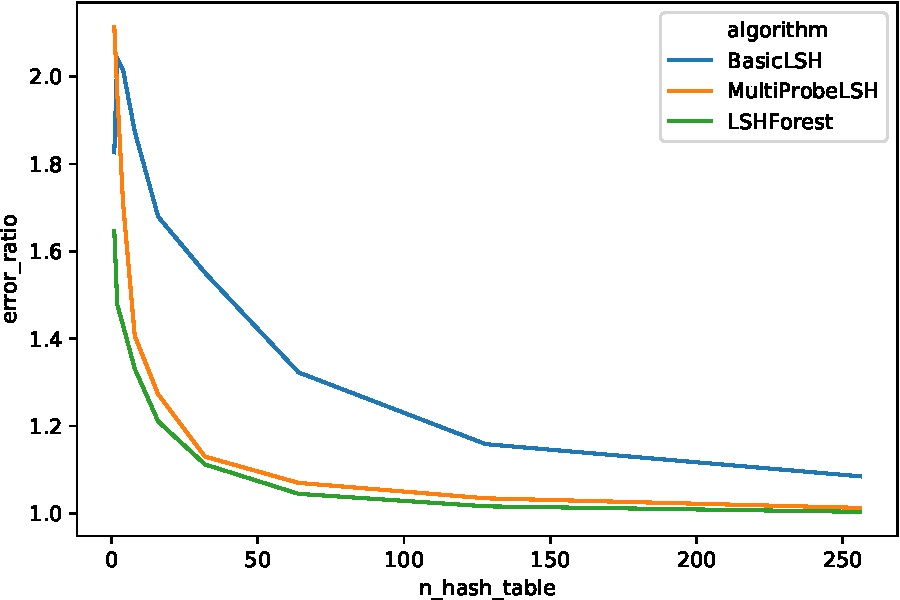
\includegraphics[width=\textwidth]{figures/error_ratio}
\end{frame}

